%!TEX root = ../acc-optim.tex
\section{Sharing recovery} % (fold)
\label{sec:sharing}

% It turns out that Emil Axelsson's Syntactic library implements typed sharing recovery using
% graphs as proposed by Gill. This is based on a graph version of Syntactic's extensible ASTs
% (and not explained in Axelsson's 2012 ICFP paper). Syntactic supports converting a graph
% with sharing backend into a tree, but it doesn't seem to support generating a let-based
% representation.
%
% How does the type safety work out in the graph representation? Are transformations really
% properly typed? 
%
% Axelsson's implementation of sharing recovery is less functional than ours. The whole process
% is in IO and, in addition to stable names, also makes use of 'IORef's.
%
% The implementation was committed July 2011: 
%   http://hub.darcs.net/emax/syntactic/patch/20110719132827-080f5
% We implemented the current version of sharing recovery in early to mid 2011 (and a preliminary
% version end of 2010).

\citet{Gill:2009dx} proposed to use \emph{stable names}~\cite{PeytonJones:StorageManager} to recover the sharing of source terms in a deeply embedded language. The stable names of two Haskell terms are equal only when the terms are represented by the same heap structure in memory. Likewise, when the abstract syntax trees (ASTs) of two terms of an embedded language have the same stable name, we know that they represent the same value. In this case we should combine them into one shared AST node. As the stable name of an expression is an intensional property, it can only be determined in Haskell's @IO@ monad.

Accelerate's runtime compiler preserves source types throughout most of the compilation process~\cite{Chakravarty:Accelerate}. In particular, it converts the source representation based on higher-order abstract syntax (HOAS) to a type-safe internal representation based on de Bruijn indices. Although developed independently, this conversion is like the \emph{unembedding} of \citet{Atkey:Unembedding}. Unembedding and sharing recovery necessarily need to go hand in hand for the following reasons. Sharing recovery must be performed on the source representation; otherwise, sharing will already have been lost. Nevertheless, we cannot perform sharing recovery on higher-order syntax as we need to traverse below the lambda abstractions used in the higher-order syntax representation. Hence, both need to go hand in hand.

As shown by \citet{Atkey:Unembedding}, the conversion of HOAS in Haskell can be implemented in a type-preserving manner with the exception of one untyped, but dynamically checked environment look up, using Haskell's @Typeable@. To preserve maximum type safety, we do not want any further operations that are not type preserving when adding sharing recovery. Hence, we cannot use Gill's algorithm. The variant of Gill's algorithm used in Syntactic~\cite{Axelsson:Syntactic} does not apply either: it (1) also generates a graph and (2) discards static type information in the process. In contrast, our novel algorithm performs simultaneous sharing recovery and conversion from HOAS to a typed de Bruijn representation, where the result of the conversion is a tree (not a graph) with sharing represented by let bindings. Moreover, it is a type-preserving conversion whose only dynamically checked operation is the same environment lookup deemed unavoidable by \citet{Atkey:Unembedding}.

In the following, we describe our algorithm using plain typed lambda terms. This avoids much of the clutter that we would incur by basing the discussion on the full Accelerate language. In addition to its implementation in Accelerate, a working Haskell implementation of our algorithm for the plain lambda calculus can be found at \url{https://github.com/mchakravarty/hoas-conv}.


% -----------------------------------------------------------------------------
\subsection{Our approach to sharing recovery}

\begin{figure*}
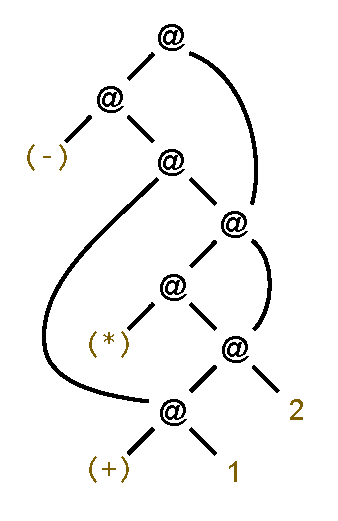
\includegraphics[scale=0.6]{figs/sharing-original.pdf}
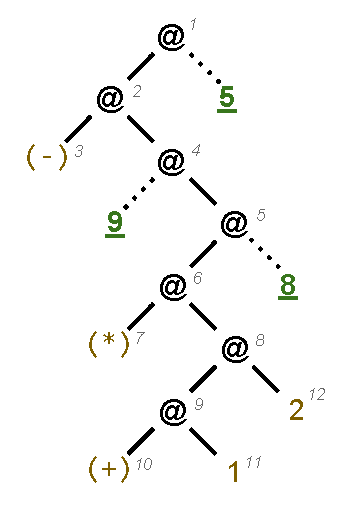
\includegraphics[scale=0.6]{figs/sharing-pruned.pdf}
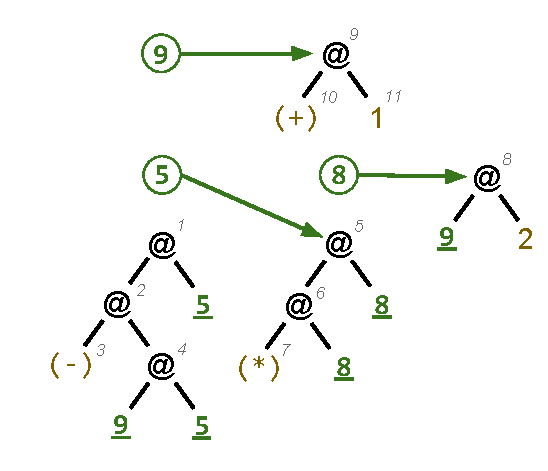
\includegraphics[scale=0.6]{figs/sharing-floated.pdf}
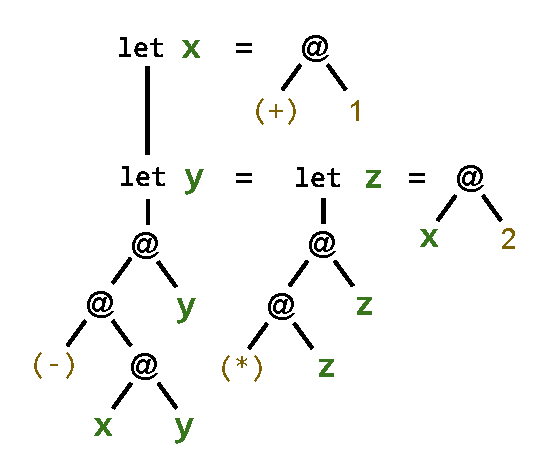
\includegraphics[scale=0.6]{figs/sharing-lets.pdf}
\caption{Recovering sharing in an example term}
\label{fig:sharing}
\end{figure*}
%
Before we formalise our sharing recovery algorithm in the following subsections, we shall illustrate the main idea. Consider the following source term:
%
\begin{quote}
\begin{code}
let    inc  = (+) 1
in let nine = let three = inc 2 
              in
              (*) three three
in
(-) (inc nine) nine
\end{code}
\end{quote}
%
This term's abstract syntax DAG is the leftmost diagram in Figure~\ref{fig:sharing}. It uses \app\ nodes to represent applications; as in this grammar:%
%
\begin{haskell*}
  T &{}\to{}& C 
  &\qquad& T^\tau \mathbf{where}\\
    &\mid   & x 
  &      &~~~C^\tau &:: T^\tau\\
    &\mid   & \lambda{x}. T 
  &      &~~~x^\tau &:: T^\tau\\
    &\mid   & T_1\app{}T_2
  &      &~~~\lambda{x^{\tau_1}}.T^{\tau_2} &:: T^{\tau_1\to\tau_2}\\
  C &\to    & \langle\text{constants}\rangle
  &      &~~~T_1^{\tau_1\to\tau_2}\app{}T_2^{\tau_1} &:: T^{\tau_2}
\end{haskell*}
%
The left definition does not track types, whereas the right one does. We implement typed ASTs in Haskell with GADTs and work with typed representations henceforth. Typed HOAS conversion with sharing recover proceeds in three stages:
%
\begin{enumerate}
  \item \emph{Prune shared subterms:} A depth first traversal over the AST annotates each node with its unique stable name, where we build an occurrence map of how many times we've already visited each node. If we encounter a previously visited node, it represents a \emph{shared subterm}, and we replace it by a placeholder containing its stable name. The second diagram in Figure~\ref{fig:sharing} shows the outcome of this stage. Each node is labeled by a number that represents its stable name, and the dotted edges indicate where we encountered a previously visited, shared node. The placeholders are indicated by underlined stable names.
  
  \item \emph{Float shared terms:} All shared subterms float upwards in the tree to just above the lowest node that dominates all edges to the original position of that shared subterm --- see the third diagram in Figure~\ref{fig:sharing}. Floated subterms are referenced by circled stable names located \emph{above} the node that they floated to. If a node collects more than one shared subterm, the subterm whose origin is deeper in the original term goes on top --- here, 9 on top of 5. Nested sharing leads to subterms floating up inside other floated subterms --- here, 8 stays inside the subterm rooted in 5.

  \item \emph{Binder introduction:} Each floated subterm gets let-bound right above the node it floated to (rightmost diagram in Figure~\ref{fig:sharing}). While we use explicit, bound names in the figure, we introduce de Bruijn indices at the same time as introducing the lets. 
\end{enumerate}


% -----------------------------------------------------------------------------
\subsection{Prune shared subterms}

First, we identify and prune shared subtrees, producing a pruned tree of the following form (second diagram in Figure~\ref{fig:sharing}):
%
\newcommand{\cT}{{^{\circ}\!T}}
\begin{haskell}
  \cT^\tau \mathbf{where} \\
  ~~~~\ell               &:: \cT^\tau
          &~& \hscom{binder conversion level}\\
  ~~~~\underline\nu^\tau  &:: \cT^\tau
          &~& \hscom{pruned subtree (name)}\\
  ~~~~C^\tau              &:: \cT^\tau \\
  ~~~~\lambda\ell.\cT^{\tau_2} &:: \cT^{\tau_1\to\tau_2} \\
  ~~~~\cT_1^{\tau_1\to\tau_2}\app{}\cT_2^{\tau_1} &:: \cT^{\tau_2} \\
\end{haskell}
% \begin{haskell*}
%   T^\circ &{}\to{}& \ell 
%           &~& \hscom{level for HOAS to de Buijn conversion}\\
%           &\mid   & \underline\nu
%           &~& \hscom{stable name of pruned shared subtree}\\
%           &\mid   & C \\
%           &\mid   & \lambda\ell. T^\circ \\
%           &\mid   & T_1^\circ\app{}T_2^\circ \\
% \end{haskell*}
%

A stable name (here, of type \<Name\>) associates a unique name with each unique term node, so that two terms with the same stable name are identical, and are represented by the same data structure in memory. Here, we denote the stable name of a term as a superscript during pattern matching --- e.g., \(1^\nu\) is a constant with stable name $\nu$, just as in the second and third diagram in Figure~\ref{fig:sharing}.

An \emph{occurrence map}, \<\Omega :: Name \mapsto Int\>, is a finite map that determines the number of occurrences of a $\textit{Name}$ that we encountered during a traversal. The expression \(\Omega\nu\) yields the number of occurrences of the name $\nu$, and we have \mbox{\(\nu\in\Omega \equiv (\Omega\nu > 0)\)}. To add an occurrence to $\Omega$, we write \(\nu\rhd\Omega\). We will see in the next subsection that we cannot simplify $\Omega$ to be merely a set of occurring names. We need the actual occurrence count to determine where shared subterms should be let-bound.

The identification and pruning of shared subtrees is formalised by the following function operating on \emph{closed} terms from \<T^\tau\>:
%
\bgroup
\hsmargin0pt
\begin{haskell}
  \hsnoalign{prune :: Level \to (Name \mapsto Int) \to T^\tau \to ((Name \mapsto Int), \cT^\tau)}
  prune \ell \Omega e^\nu &\mid \nu\in\Omega &= (\nu\rhd\Omega, \underline\nu) \\
  prune \ell \Omega e^\nu &\mid otherwise    &= enter (\nu\rhd\Omega) e
  \hswhere{
    enter \Omega c                &= (\Omega, c) \\
    enter \Omega (\lambda{x}.e)   &= \hslet{(\Omega', e') = prune (\ell+1) \Omega ([\ell/x]e)}{(\Omega', \lambda\ell.e')} \\
    enter \Omega ({e_1}\app{e_2}) &= 
      \hslet{
          (\Omega_1, e_1') = prune \ell \Omega e_1 \\
          (\Omega_2, e_2') = prune \ell \Omega_1 e_2
        }{
          (\Omega_2, {e_1'}\app{e_2'})
        } \\
  }
\end{haskell}
\egroup
%
% \ben{We can't perform the substitution $[\ell/x]e$ because while $e$ has type $T$, $\ell$ has type $\cT$. We'd instead need to keep a map of $Vars \mapsto Levels$ and update this on the way down.}
% As this is HOAS, we cannot have a map of $Vars \mapsto Levels$ either. Instead, we have $\ell$ already in $T$ in the Haskell implementation. Even more precisely, we don't have $[\ell/x]e$, but the $\lambda$ is a really Haskell function and we apply it to $\ell$. Doing this exactly as in Haskell would add clutter and additional explanation. As we are doing the morally right thing here, I think, it is ok to leave it as it is.
%
The first equation of \<prune\> covers the case of a term's repeated occurrence. In that case, we prune sharing by replacing the term \<e^\nu\> by a tag \<\underline\nu\> containing its stable name --- these are the dotted lines in the second diagram in Figure~\ref{fig:sharing}.

To interleave sharing recovery with the conversion from HOAS to typed de Bruijn indices, \<prune\> tracks the nesting \<Level\> of lambdas. Moreover, the lambda case of \<enter\> replaces the HOAS binder \<x\> by the level \<\ell\> at the binding and usage sites.

Why don't we separate computing occurrences from tree pruning? When computing occurrences, we must not traverse shared subtrees multiple times, so we can as well prune at the same time. Moreover, in the first line of \<prune\>, we cannot simply return \<e\> instead of \<\underline\nu\> --- \<e\> is of the wrong form as it has type \<T\> and not \<\cT\>! 

As far as type-preservation is concerned, we do lose information due to replacing variables by levels $\ell$. This is the inevitable loss described by \citet{Atkey:Unembedding}, which we make up for by a dynamic check in an environment lookup, as already discussed.

% We could not enter shared subtrees multiple times and still leave pruning to the following stage. This has some advantages and some disadvantages (need to use the occurrences map in the next round again to spot shared subtrees). There seems to be no one undisputedly best decomposition here.


% -----------------------------------------------------------------------------
\subsection{Float shared subterms}

Second, we float all shared subtrees out to where they should be let-bound, represented by (see third diagram in Figure~\ref{fig:sharing})
%
\newcommand{\uT}{{^\uparrow\!T}}
\newcommand{\dT}{{^\downarrow\!T}}
\begin{haskell}
  \hsnoalign{\uT^\tau {}\to{} \overline{\nu : \uT^{\tau'}} \succ \dT^\tau}
  \dT^\tau \mathbf{where} \\
  ~~~~\underline\nu^\tau  &:: \dT^\tau \\
  ~~~~C^\tau              &:: \dT^\tau \\
  ~~~~\lambda\nu.\uT^{\tau_2} &:: \dT^{\tau_1\to\tau_2} \\
  ~~~~\uT_1^{\tau_1\to\tau_2}\app{}\uT_2^{\tau_1} &:: \dT^{\tau_2} \\
\end{haskell}
% \begin{haskell*}
%   T^\uparrow &{}\to{}& \overline{\nu : T^\uparrow} \succ T^\downarrow \\
%   T^\downarrow
%           &{}\to{}& \underline\nu \\
%           &\mid   & C \\
%           &\mid   & \lambda\nu. T^\uparrow \\
%           &\mid   & T_1^\uparrow\app{}T_2^\uparrow \\
% \end{haskell*}
%
A term in \<\uT\> comprises a sequence of floated-out subterms labelled by their stable name as well as a body term from \<\dT\> from which the floated subterms where extracted. Moreover, the levels \<\ell\> that replaced lambda binders in \<\cT\> get replaced by the stable name of their term node. This simplifies a uniform introduction of de Bruijn indices for let and lambda bound variables. 

We write \<\overline{\nu : \uT}\> for a possibly empty sequence of items: \<\nu_1 : \uT_1, \ldots, \nu_n : \uT_n\>, where $\bullet$ denotes an empty sequence. 
%When the sequence of floated subterms is empty we sometimes write just \<T^\downarrow\> as shorthand for \<{\bullet}\succ{T^\downarrow}\>.
% Really? Where?

The floating function \<float\> maintains an auxiliary structure of floating terms and levels, defined as follows:
%
% \begin{haskell*}
%   \Gamma &{}\to{}& \float\nu{i}{T^\uparrow} &~&\hscom{floated shared subtree} \\
%          &\mid   & \float\nu{i}\cdot        &~&\hscom{floated pruned subtree} \\
%          &\mid   & \float\nu{i}\ell         &~&\hscom{floated level tag} \\
% \end{haskell*}
\begin{haskell*}
  \Gamma &{}\to{}& \float\nu{i}{\uT^\tau} 
          {}\mid{} \float\nu{i}\cdot
          {}\mid{} \float\nu{i}\ell
\end{haskell*}
%
These are floated subtrees named \<\nu\> of which we have collected $i$ occurrences. The occurrence count indicates where a shared subterm gets let bound: namely at the node where it matches \<\Omega\nu\>. This is why \<prune\> needed to collect the number of occurrences in \<\Omega\>. When the occurrence count matches \<\Omega\nu\>, we call the floated term \emph{saturated}. The following function determines saturated floated terms, which ought to be let bound:
%
\begin{haskell}
  \hsnoalign{bind :: (Name \mapsto Int) \to \overline\Gamma \to \overline{\exists\tau.\nu : \uT^\tau}}
  bind \Omega \bullet                             &= \bullet \\
  bind \Omega (\float\nu{i}e, \overline\Gamma)
    \mid \Omega\nu == i                           &= \nu:e, bind \Omega \overline\Gamma \\
  bind \Omega (\float\nu{i}\_, \overline\Gamma)   &= bind \Omega \overline\Gamma
\end{haskell}
%
Note that \<\Gamma\> does not keep track of the type \<\tau\> of a floated term \<\uT^\tau\>; hence, floated terms from \<bind\> come in an existential package. This does \emph{not} introduce additional loss of type safety as we already lost the type of lambda bound variables in \<\float\nu{i}\ell\>. It merely means that let bound, just like lambda bound, variables require the dynamically checked environment look up we already discussed.

When floating the \emph{first occurrence} of a shared tree (not pruned by \<prune\>), we use \<\float\nu{i}{\uT^\tau}\>. When  floating \emph{subsequent occurrences} (which were pruned), we use \<\float\nu{i}\cdot\>. Finally, when floating a level, to replace it by a stable name, we use \<\float\nu{i}\ell\>.

We define a partial ordering on floated terms: \<\float{\nu_1}{i}{x} < \float{\nu_2}{j}{y}\> iff the direct path from \<\nu_1\> to the root of the AST is shorter than that of \<\nu_2\>. We keep sequences of floated terms in \emph{descending order} --- so that the deepest subterm comes first. We write \<\overline{\Gamma_1}\uplus\overline{\Gamma_2}\> to merge two sequences of floated terms. Merging respects the partial order, and it combines floated trees with the same stable name by adding their occurrence counts. To combine the first occurrence and a subsequent occurrence of a shared tree, we preserve the term of the first occurrence. We write \<\overline\Gamma\setminus\overline\nu\> to delete elements of \<\overline\Gamma\> that are tagged with a name that appears in the sequence \<\overline\nu\>.

We can now formalise the floating process as follows:
%
\begin{haskell}
  \hsnoalign{float :: (Name \mapsto Int) \to \cT^\tau \to (\overline\Gamma, \uT^\tau)}
  float \Omega \ell^\nu      &= (\float\nu{1}\ell,  \underline\nu)\\
  float \Omega \underline\nu &= (\float\nu{1}\cdot, \underline\nu)\\
  float \Omega e^\nu         &= 
  \hslet{
    (\overline\Gamma, e')    &= descend e \\
    \overline{\nu_b : e_b}   &= bind \Omega \overline\Gamma \\
    d                        &= \overline{\nu_b : e_b} \succ e'
  }{%
    \hsif{
      \Omega\nu == 1
    }{
      (\overline\Gamma\setminus\overline{\nu_b}, d)  
    }{
      \hsalign{
        (\overline\Gamma\setminus\overline{\nu_b}\uplus\{\nu:d\}, \underline\nu)
      }
    }
  }
  \hswhere{
    \hsnoalign{descend :: \cT^\tau \to (\overline\Gamma, \dT^\tau)}
    descend c               &= (\bullet, c)\\
    descend (\lambda\ell.e) &= 
      \hslet{
        (\overline\Gamma, e') = float \Omega e
      }{
        \hsif{
          \exists \nu' i. (\float{\nu'}{i}\ell)\in\overline\Gamma
        }{
          (\overline\Gamma\setminus\{\nu'\}, \lambda\nu'.e')
        }{
          (\overline\Gamma, \lambda\_.e')
        }
      }\\
    descend ({e_1}\app{e_2}) &= 
      \hslet{
        (\overline\Gamma_1, e_1') = float \Omega e_1 \\
        (\overline\Gamma_2, e_2') = float \Omega e_2
      }{
        (\overline\Gamma_1\uplus\overline\Gamma_2, {e_1'}\app{e_2'})
      }
  }
\end{haskell}
%
The first two cases of \<float\> ensure that the levels of lambda bound variables and the names of pruned shared subterms are floated regardless of how often they occur. In contrast, the third equation floats a term with name $\nu$ only if it is shared; i.e., \<\Omega\nu\> is not 1. If it is shared, it is also pruned; i.e., replaced by its name \<\underline\nu\> --- just as in the third diagram of Figure~\ref{fig:sharing}.

Regardless of whether a term gets floated, all saturated floated terms, \<\overline{\nu_b : e_b}\>, must prefix the result, \<e'\>, and be removed from \<\overline\Gamma\>.

When \<descend\>ing into a term, the only interesting case is for lambdas. For a lambda at level \<\ell\>, we look for a floated level of the form \<\nu':\ell\>. If that is available, \<\nu'\> replaces \<\ell\> as a binder and we remove \<\nu':\ell\> from \<\overline\Gamma\>. However, if \<\nu':\ell\> is not in \<\overline\Gamma\>, the binder introduced by the lambda doesn't get used in \<e\>. In this case, we pick an arbitrary new name; here symbolised by an underscore ''\<\_\>''.


% -----------------------------------------------------------------------------
\subsection{Binder introduction}

Thirdly, we introduce typed de Bruijn indices to represent lambda and let binding structure (rightmost diagram in Figure~\ref{fig:sharing}):
%
\newcommand{\iT}[1][env]{{^{#1}\!T}}
\newcommand{\idx}[1][env]{{^{#1}\!\iota}}
\begin{haskell}
  \iT^\tau \mathbf{where} \\
  ~~~~C^\tau              &:: \iT^\tau \\
  ~~~~\idx^\tau           &:: \iT^\tau \\
  ~~~~\lambda{\iT[(\tau_1, env)]^{\tau_2}} &:: \iT^{\tau_1\to\tau_2} \\
  ~~~~\iT_1^{\tau_1\to\tau_2}\app{}\iT_2^{\tau_1} &:: \iT^{\tau_2} \\
  ~~~~\letin{\iT_1^{\tau_1}}{\iT[(\tau_1, env)]_2^{\tau_2}} &:: \iT^{\tau_2} \\
\end{haskell}
% \begin{haskell*}
%   T^\iota &{}\to{}& C \\
%           &\mid   & \iota \\
%           &\mid   & \lambda{T^\iota} \\
%           &\mid   & T_1^\iota\app{}T_2^\iota \\
%           &\mid   & \letin{T_1^\iota}{T_2^\iota} \\
% \end{haskell*}
%
With this type of terms, \<e::\iT^\tau\> means that \<e\> is a term representing a computation producing a value of type \<\tau\> under the type environment \<env\>. Type environments are nested pair types, possibly terminated by a unit type \<()\>. For example, \<(((), \tau_1), \tau_0)\> is a type environment, where de Bruijn index 0 represents a variable of type \<\tau_0\> and de Bruijn index 1 represents a variable of type \<\tau_1\>.

We abbreviate \<\mathtt{let} e_1 \mathtt{in} \cdots \mathtt{let} e_n \mathtt{in} e_b\> as \<\letin{\overline{e}}{e_b}\>. Both \<\lambda\> and \<\mathtt{let}\> use de Bruijn indices \<\iota\> instead of introducing explicit binders.

To replace the names of pruned subtrees and of lambda bound variables by de Bruijn indices, we need to construct a suitable type environment as well as an association of environment entries, their de Bruijn indices, and the stable names that they replace. We maintain the type environment with associated de Bruijn indices in the following \emph{environment layout} structure:
%
\newcommand{\Lyt}[1][env]{{^{#1}\!\Delta}}
\begin{haskell}
  \Lyt^{env'} \hskwd{where} \\
  ~~~~\circ &:: \Lyt^{()} \\
  ~~~~\Lyt^{env'};\idx^\tau &:: \Lyt^{(env', t)} \\
\end{haskell}
%
Together with a layout, we use a sequence of names \<\overline\nu\> of the same size as the layout, where corresponding entries represent the same variable. As this association between typed layout and untyped sequence of names is not validated by types, the lookup function \<lyt\mathrel\downarrow{i}\> getting the $i$th index of layout \<lyt\> makes use of a dynamic type check. It's signature is \<(\downarrow) :: \mathbb{N} \to \Lyt^{env'} \to \idx^\tau\>.

Now we can introduces de Bruijn indices to body expressions:
%
\begin{haskell}
  \hsnoalign{body :: \Lyt^{env} \to \overline\nu \to \dT^\tau \to \iT^\tau}
  \hsnoalign{body\hsap lyt\hsap (\nu_{\rho,0}, \ldots, \nu_{\rho,n})\hsap \underline\nu} \\
    ~~\mid \nu == \nu_{\rho,i} &= lyt\mathrel\downarrow{i} \\
  body lyt \overline{\nu_\rho} c
    &= c \\
  body lyt \overline{\nu_\rho} (\lambda\nu.e)
    &= \lambda(binders lyt^+ (\nu,\overline{\nu_\rho}) e) \\
  body lyt \overline{\nu_\rho} (e_1\app{e_2})
    &= (binders lyt \overline{\nu_\rho} e_1)\app(binders lyt \overline{\nu_\rho} e_2)
\end{haskell}
%
The first equation performs a lookup in the environment layout at the same index where the stable name \<\nu\> occurs in the name environment \<\overline\nu\>. The lookup is the same for lambda and let bound variables. It is the only place where we need a dynamic type check and that is already needed for lambda bound variables alone.

In the case of a lambda, we add a new binder by extending the layout, denoted \<lyt^+\>, with a new zeroth de Bruijn index and shifting all others one up. Keeping the name environment in sync, we add the stable name \<\nu\>, which \<\dT\> used as a binder.

In the same vein, we bind $n$ floated terms \<\overline{\nu:e}\> with \<\mathtt{let}\> bindings in body expression \<e_b\>, by extending the type environment $n$ times (\<map\> applies a function to each element of a sequence):
%
\begin{haskell}
  \hsnoalign{binders :: \Lyt^{env} \to \overline\nu \to \uT^\tau \to \iT^\tau}
  binders lyt \overline{\nu_\rho} (\overline{\nu:e} \succ e_b) =
  \hsbody{
     \letin{map (binders lyt \overline{\nu_\rho}) \overline{e}}{body lyt^{+n} (\overline\nu,\overline{\nu_\rho}) e_b}
  }\\
  \hsap\hskwd{where} n = length (\overline{\nu:e})
\end{haskell}
%
We tie the three stages together to convert from HOAS with sharing recovery producing let bindings and typed de Bruijn indices:
%
\begin{haskell}
  hoasSharing :: T^\tau \to \iT[()]^\tau \\
  hoasSharing e = 
    \hslet{
      (\Omega, e')   &= prune 0 \bullet e \\
      (\bullet, e'') &= float \Omega e'
    }{
      binders {\circ} \bullet e''
    }
\end{haskell}

% section sharing (end)
